\begin{figure}[t]\centering
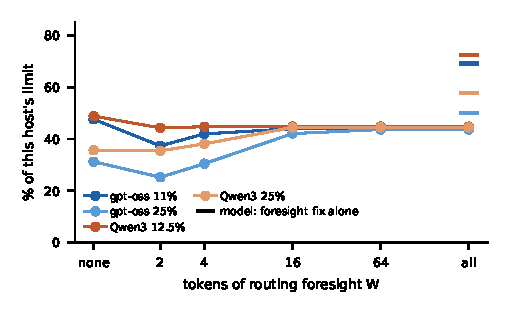
\includegraphics[width=\linewidth]{figs/foresight.pdf}
\caption{Foresight in the engine, measured on another rented RTX 5090 (Ryzen 9 9950X): speed as a percentage of this
host's limit against the window $W$ of future routing the hit-optimal oracle sees, at the four host-bound cells.
``none'' is the online policy; ``all'' the whole sequence; points are connected for the trend only. The tick at the
right is the accounting's foresight-only term for the cell, the speed the model predicts with that one fix.}
\label{fig:foresight}
\end{figure}

\paragraph{Foresight, measured.} We then gave the engine foresight of future routing, in two forms, and measured what
each is worth. An oracle policy reads the routing of the next $W$ decode steps from a trace recorded on the same
machine over the same teacher-forced text; its copies ride the paced admission path (16\,MB pieces; pacing the online
policy itself changes it by under 1\%), and an expert still in flight at its step runs on the CPU like any other
miss. The \emph{hit-optimal} oracle admits the experts those steps will route to, soonest first, evicting the resident
whose next use is furthest (Belady within the window); it admits an expert for one future use as readily as for ten.
The \emph{bytes-optimal} oracle is the policy whose reads define the limit, MIN with bypass: a miss runs on the CPU
and is admitted only if its next use comes before the furthest next use among the residents, which it then evicts.
Each ran on a rented RTX 5090 host with weak host memory (a Ryzen 9 9950X and a Ryzen 9 7950X, both reading
\fsmHostCpu--\fsbHostCpu\,GB/s by the CPU and \fsmHostLink--\fsbHostLink{} over the link; \cref{fig:foresight},
\cref{app:foresight}). With the whole sequence in view the hit-optimal oracle runs \fsmRatioGMid$\times$
[\fsmRatioLoGMid, \fsmRatioHiGMid] the online policy at gpt-oss 25\% and \fsmRatioQMid$\times$ [\fsmRatioLoQMid,
\fsmRatioHiQMid] at Qwen3 25\% on the first host, \fspRatioGMid$\times$ and \fspRatioQMid$\times$ on the second, and
\fsmRatioGHigh--\fspRatioQHigh$\times$ at the two GPU-bound cells; half of the gain at gpt-oss 25\% arrives between
$W{=}4$ and 16 (\fsmWfiftyGMid{} tokens by log interpolation), near the 10 its trace gives in \cref{sec:traces}.
Where the host binds hardest it \emph{loses}, \fspLossMin--\fsmLossMax\% at gpt-oss 11\% and Qwen3 12.5\% on both
hosts, and at every window on the first: it reads more host bytes than the online policy (\fsmReadsOracleGLow{} and
\fsmReadsOracleQLow{} experts per token, misses plus admissions, against \fsmReadsBaseGLow{} and \fsmReadsBaseQLow),
because Belady admits an expert used once where the optimum, at \fsmReadsOptGLow{} and \fsmReadsOptQLow{} reads per
token, bypasses it. The bytes-optimal oracle gains \fsbGainHighMin--\fsbGainHighMax\% at the four cells of 25\% and
above and \fsbGainLowMin--\fsbGainLowMax\% at the two below, and the law on its own counters predicts its time within
\fsbLawErrMax\%: fewer host bytes, the mechanism the accounting's foresight term describes, and nothing else. Its
reads fall (\fsbMissesBaseGMid{} to \fsbMissesGMid{} and \fsbMissesBaseQMid{} to \fsbMissesQMid{} misses per token at
25\%) but stay \fsbReadsRatioMin--\fsbReadsRatioMax$\times$ the optimum's, because a copy lands two to three steps
after it is issued and the expert misses again meanwhile: the same policy simulated on the trace reproduces the
engine's misses at a copy latency of \fslFitHostMin--\fslFitHostMax{} steps at the host-bound cells and comes within
\fslIdealOverMin--\fslIdealOverMax\% of the optimum's reads at one (\cref{tab:foresight_bytes}). The hit-optimal oracle, which reads as many host bytes as the
online policy, gains \fspGainHighMin--\fspGainHighMax\% at the same four cells on the same host, and the law, with
its GPU term calibrated on the online run, over-predicts those runs by \fspLawErrHighMin--\fspLawErrHighMax\%: its
gain is the overlap of copies issued ahead of their use with the step, which the law charges in sequence. In this
engine, then, the accounting's two largest terms are one mechanism. The bytes foresight saves are worth
\fsbGainHighMin--\fsbGainHighMax\% where the link has slack; the rest of foresight's measured value is the overlap it
makes possible, and where the host binds hardest neither form gains more than \fsbGainLowMax\%. The engine's
within-layer overlap of a layer's CPU misses with its GPU hits, turned off, changes speed by under 1\% at every cell,
so the overlap the accounting charges is across the step, not within a layer.
